\ifdefined\beamerclass
\else
    \def\beamerclass{beamer}
\fi
\documentclass[\beamerclass]{beamer}

\usepackage{pgfpages}
\mode<handout>{
	% \setbeamercolor{background canvas}{bg=black!20}
	\pgfpagesuselayout{2 on 1}[a4paper,border shrink=5mm]
}

\usepackage{lmodern}
\usepackage{listings}
\usepackage{amsmath}
\usepackage{bm}
\usepackage{textpos} % package for the positioning

\usepackage{pgf, tikz}
\usetikzlibrary{arrows, automata}

\usetheme{Copenhagen}
\hypersetup{pdfstartview={Fit}}
\lstset{basicstyle=\small\ttfamily,breaklines=true}

\title[COMP6248 Deep Learning]{COMP6248 Differentiable Programming}
\subtitle{(and some Deep Learning)}
\author{Kate Farrahi and Jonathon Hare}
\institute[]
{
  Vision, Learning and Control\\
  University of Southampton 
}
\date{}
\subject{Computer Science}
\useoutertheme{infolines}
\setbeamertemplate{headline}{} %remove headline
\setbeamertemplate{navigation symbols}{} %remove navigation symbols

\begin{document}
  \frame{
  \titlepage
}

\begin{frame}{pause}
\frametitle{Machine Learning - A Recap}
{\tiny All credit for this slide goes to Niranjan}\\
\vspace{5mm}
\begin{tabular}{ll}
Data & $\{\bm{x}_n, \bm{y}_n\}^N_{n=1} \qquad \{\bm{x}_n\}^N_{n=1}$ 
\vspace{3mm} \\ \pause
Function Approximator & $\bm{y} = f (\bm{x}, \bm{\theta}) + \nu$ 
\vspace{3mm} \\ \pause
Parameter Estimation & $E_0 = \sum^N_{n=1} \{\|\bm{y}_n - f (\bm{x}_n; \bm{\theta})\|\}^2$
\vspace{3mm} \\ \pause
Prediction & $\bm{\hat y}_{N+1} = f(\bm{x}_{N+1}, \bm{\hat \theta})$
\vspace{3mm} \\ \pause
Regularisation & $E_1 = \sum^N_{n=1} \{\|\bm{y}_n - f (\bm{x}_n; \bm{\theta})\|\}^2 + r(\|\bm\theta\|)$
\vspace{3mm} \\ \pause
Modelling Uncertainty & $p(\bm\theta|\{\bm x_n, \bm y_n\}_{n=1}^N)$
\vspace{3mm} \\ \pause
Probabilistic Inference & $\mathop{\mathbb{E}}[g(\bm\theta)] = \int g(\bm\theta)p(\bm\theta)d\bm\theta = \frac{1}{N_s}\sum_{n=1}^{N_s}g(\bm\theta^{(n)})$
\vspace{3mm} \\ \pause
Sequence Modelling & $\bm x_n = f(\bm x_{n-1}, \bm\theta)$
\end{tabular}
\vspace{5mm}
\end{frame}

\begin{frame}
\frametitle{What is Deep Learning?}

Deep learning is primarily characterised by function compositions: \\ \vspace{10mm}
\begin{itemize}
	\item<+-> Feedforward networks: $\bm{y} = f (g(\bm{x}, \bm\theta_g), \bm{\theta_f})$
	\begin{itemize}
		\item Often with relatively simple functions (e.g. $f(\bm x, \bm{\theta}_f) = \sigma(\bm{x}^\top \bm{\theta}_f)$)
	\end{itemize} \vspace{3mm}
	\item<+-> Recurrent networks: $\bm y_t = f(\bm y_{t-1}, \bm x_t, \bm\theta) = f(f(\bm y_{t-2}, \bm x_{t-1}, \bm\theta), \bm\theta) = \dots$
\end{itemize}
\vspace{10mm}

\uncover<+->{
In the early days the focus of deep learning was on learning functions for classification. Nowadays the functions are much more general in their inputs and outputs.
}

\end{frame}

\begin{frame}
\frametitle{What is Differentiable Programming?}
	
\begin{itemize}
	\item<+-> Differentiable programming is a term coined by Yann Lecun\footnote{https://www.facebook.com/yann.lecun/posts/10155003011462143} to describe a superset of Deep Learning.
	\item<+-> Captures the idea that computer programs can be constructed of parameterised functional blocks in which the parameters are learned using some form of gradient-based optimisation.
	\begin{itemize}
		\item<+-> The implication is that we need to be able to compute gradients with respect to the parameters of these functional blocks. We'll start explore this in detail next week...
		\item<+-> The idea of Differentiable Programming also opens up interesting possibilities: 
		\begin{itemize}
			\item The functional blocks don't need to be direct functions in a mathematical sense; more generally they can be \emph{algorithms}.
			\item What if the functional block we're learning parameters for is itself an algorithm that optimises the parameters of an internal algorithm using a gradient based optimiser?!\footnote{See our ICLR 2019 paper: https://arxiv.org/abs/1812.03928}
		\end{itemize}
	\end{itemize}
\end{itemize}
\end{frame}

\begin{frame}
\frametitle{Is all Deep Learning Differentiable Programming?}
\begin{itemize}
	\item Not necessarily!
	\begin{itemize}
		\item<+-> Most deep learning systems are trained using first order gradient-based optimisers, but there is an active body of research on gradient-free methods.
		\item<+-> There is an increasing interest in methods that use different styles of learning, such as Hebbian learning, within deep networks. More broadly there are a number of us\footnote{including at least myself, my PhD students and Geoff Hinton!} who are interested in biologically motivated models and learning methods.
	\end{itemize}
\end{itemize}
\end{frame}

\begin{frame}
	\frametitle{Why should we care about this?}
	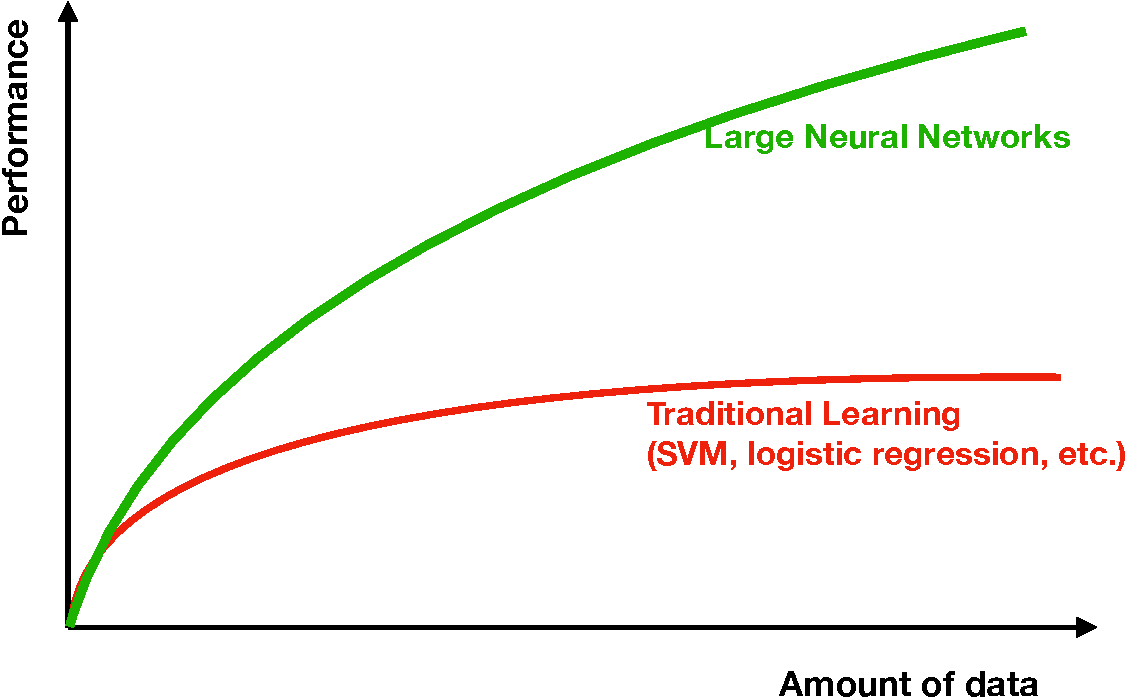
\includegraphics[width=0.9\textwidth]{Fig1.pdf}\footnote{Reference: Andrew Ng}
\end{frame}

\begin{frame}
	\frametitle{Where did it all start \& what was the motivation?}
	
\end{frame}

\begin{frame}
	\frametitle{What is the objective of this module?}
	\begin{enumerate}
		\item To gain an in-depth theoretical and practical understanding of modern deep neural networks and their applications.
		\item Understand the underlying mathematical and algorithmic principles of deep learning
		\item Understand the key factors that have made deep learning successful for various applications
		\item Apply existing deep learning models to real datasets
		\item Gain facility in working with deep learning libraries in order to create and evaluate network architectures
		\item Critically appraise the merits and shortcomings of model architectures on specific problems
	\end{enumerate}
\end{frame}


\begin{frame}
	\frametitle{What will we cover in the module?}
	\url{http://comp6248.ecs.soton.ac.uk/}
\end{frame}

\begin{frame}
	\frametitle{How is this module going to be delivered?}
	
	\begin{enumerate}
	\item Reading material before the lectures
	\end{enumerate}
\end{frame}

\begin{frame}
	\frametitle{Lab session plan}
	
	\begin{center}
	\begin{tabular}{ c c c }
		 Lab & Date & Topic \\ \hline
		 Lab 1 &  05/02/19 & Introducing PyTorch \\ 
		 Lab 2 & 12/02/19 & Automatic Differentiation \\  
		 Lab 3 & 19/02/19 & Optimisation   \\
		 Lab 4 & 26/02/19 & NNs with PyTorch and Torchbearer   \\
 		Lab 5 & 05/03/19 & CNNs with PyTorch and Torchbearer   \\
 		Lab 6 & 12/03/19 & Transfer Learning \\
 		Lab 7 & 19/03/19 & RNNs, Sequence Prediction and Embeddings \\
		 Lab 8 & 26/03/19 & Deep Generative Models\\ \hline 
		 & Break & \\
		 \hline
		 Lab 9 & 30/04/19 & Coursework Help and Advice \\
		 Lab 10 & 30/04/19 & Coursework Help and Advice \\
 		 Lab 11 & 30/04/19 & Coursework Help and Advice \\
	\end{tabular}
	\end{center}
\end{frame}

\begin{frame}
	\frametitle{What do we expect you already know?}
	
	\begin{enumerate}
	\item COMP3206 or COMP3223 or COMP6229 or COMP6245
	\item Fundamentals of Linear Algebra, Probability and Statistics, Calculus
	\item Programming in Python
	\end{enumerate}
\end{frame}

%\begin{frame}
%	\frametitle{What might you already know?}	
%\end{frame}

\begin{frame}
	\frametitle{Assessment Structure}
	\begin{enumerate}
		\item Lab work $40\%$
		\item Final project $40\%$ \\  
		\item In-class tests $20\%$ \\	
	\end{enumerate}
\end{frame}

\begin{frame}
	\frametitle{Assessment Timetable}
	
	\begin{center}
	\begin{tabular}{ l c  c}
		 Assessment & Date  & Time\\ \hline
		 Labs 1-3  &  22/02/19 & 16:00 \\ 
		 Coursework Team Information & 27/02/19 & 16:00 \\
		 In - class Test 1 & 01/03/19 & midnight  \\		 
		 Labs 4-6  & 15/03/19 & 16:00 \\  
		 In - class Test 2 & 29/03/19 & midnight  \\		 
		 Labs 7-8 & 03/05/19 & 16:00   \\
		 Final Coursework Submission & 15/05/19 & 16:00 \\
	\end{tabular}
	\end{center}
	
\end{frame}

\begin{frame}
	\frametitle{The Main Assignment}
	\framesubtitle{The ICLR Reproducibility Challenge}
	\url{http://comp6248.ecs.soton.ac.uk/coursework.html}
	
\end{frame}

\end{document}